% CS 412 Final Project Report -- CVPR author-kit template (https://github.com/cvpr-org/author-kit)
\documentclass[10pt,twocolumn,letterpaper]{article}

\usepackage[pagenumbers]{cvpr}
\usepackage{amsthm,amsfonts,mathtools,bm,multirow}
\usepackage{microtype}

\definecolor{cvprblue}{rgb}{0.21,0.49,0.74}
\usepackage[breaklinks,colorlinks,allcolors=cvprblue]{hyperref}

\def\confName{CS 412}
\def\confYear{2026}

% ---------- macros ----------
\newcommand{\vx}{\mathbf{x}}
\newcommand{\vz}{\mathbf{z}}
\newcommand{\vb}{\mathbf{b}}
\newcommand{\valpha}{\boldsymbol{\alpha}}
\newcommand{\vmu}{\boldsymbol{\mu}}
\newcommand{\veps}{\boldsymbol{\epsilon}}
\newcommand{\E}{\mathbb{E}}
\newcommand{\real}{\mathbb{R}}
\newcommand{\cS}{\mathcal{S}}
\newcommand{\cJ}{\mathcal{J}}
\newcommand{\cL}{\mathcal{L}}
\newcommand{\TODO}[1]{{\color{red}[TODO: #1]}}
\newcommand{\para}[1]{\textit{#1.}}

\newtheorem{theorem}{Theorem}
\newtheorem{proposition}{Proposition}
\theoremstyle{definition}
\newtheorem{definition}{Definition}
\newtheorem{assumption}{Assumption}

\title{Causal Representation Learning in Dynamic Environments:\\Tracking Mechanism Transitions and Interpreting Regime Changes}

\author{Shicheng Fan \qquad Jie Yang \qquad Honghui Bao\\
University of Illinois Chicago\\
{\small CS 412 Final Project Report, Fall 2026}
}

\begin{document}
\maketitle

% =====================================================================
\begin{abstract}
Causal representation learning (CRL) recovers the latent variables behind high-dimensional observations.
In a dynamic environment the mechanism that governs these latents changes over time: a vehicle enters a turn, a molecule unfolds as it is heated, a climate system moves between phases.
Current temporal CRL uses such changes only as a signal that makes the latents identifiable.
It treats the environment as a handful of discrete regimes, and it leaves the recovered latents without a meaning.
This project studies two aspects of the change that remain open once the latents are identified.
The first is the transition itself.
We model a gradual transition as a path of convex combinations of a few atomic mechanisms and recover the path at test time with a least-squares readout, for which we give an error bound.
The second is the meaning of the change.
We attach to each latent a sparse set of named observed variables through an additive decoder, and show that these sets are identifiable, so the latent that differs most between two regimes can be read as a physical module.
Both parts share one design: identify the latents first, then apply a simple readout that can be analyzed on its own.
Experiments on controlled benchmarks, vehicle motion, and molecular dynamics support both parts.
\end{abstract}

% =====================================================================
\section{Introduction}
\label{sec:intro}

Causal representation learning (CRL)~\cite{scholkopf2021toward,zhang2024causal} aims to recover, uniquely, the latent variables that generate high-dimensional observations.
The property is called \emph{identifiability}: two models that explain the data equally well must agree on the latents, up to a permutation and a component-wise invertible map.
For nonlinear models this is impossible without extra structure~\cite{hyvarinen1999nonlinear,locatello2019challenging}.
Time series supply that structure.
If the dynamics of the latents differ across regimes, the differences pin the latents down~\cite{hyvarinen2016unsupervised,yao2022temporally}.

In other words, existing methods need the environment to change, but they treat the change itself as a nuisance label.
The environment is assumed to sit in one of a few discrete regimes, the regime index is used as an auxiliary variable during training, and nothing more is said about it.
For a system that really is dynamic, this leaves out two things.

The first is the transition itself.
Real transitions are rarely instantaneous.
A vehicle moves gradually from straight driving into a turn, and a person passes through intermediate gaits between walking and running.
A model with discrete regimes can only say which regime is closest; it cannot say how far along the transition the system is, and it cannot represent an intermediate state it has never seen.

The second is the meaning of the change.
Even when the latents are identified, each one is an anonymous coordinate.
In scientific data the hidden mechanism is exactly what we are trying to discover, so there is no ground truth to match the latents against.
What we do have is named observations: residue distances in a molecule, sea-surface temperatures, process sensors.
If we knew which named observations a latent drives, the latent that moves when the regime changes would have a physical reading.

This project studies both aspects in one framework (Fig.~\ref{fig:simplex}, Table~\ref{tab:compare}).
The latents follow a temporal process whose transition law depends on a mechanism state.
A first stage learns identifiable latents from regime-dependent dynamics, as in prior work.
A second stage adds a readout to the frozen representation, one for each aspect:
\begin{itemize}
\item Tracking (Sec.~\ref{sec:track}).
The mechanism state is a point in a simplex spanned by a few atomic mechanisms.
A least-squares projection of the latent dynamics onto a learned basis recovers the time-varying mixing weights.
\item Interpreting (Sec.~\ref{sec:interp}).
Given two regimes, for instance the two ends of a transition, an additive sparse decoder recovers which observed variables each latent drives.
\end{itemize}
Because each readout is simple, it can be analyzed.
We show that the mixing trajectory is recovered with an explicit error bound, and that the observation supports of the latents are identifiable.

The experiments support both parts.
On synthetic transitions, tracking reaches a correlation of $0.94$ with the true mixing trajectory, against $0.72$ for the best discrete-switching baseline.
On a real vehicle turn it reaches $0.96$ against $0.24$.
For interpretation, on a benchmark with known supports our decoder reaches a support precision of $0.978$ where dense decoders score zero, and on RNA and protein molecular dynamics the latent that moves with the regime lands on the structural region that the regime was defined on.

\begin{figure}[t]
\centering
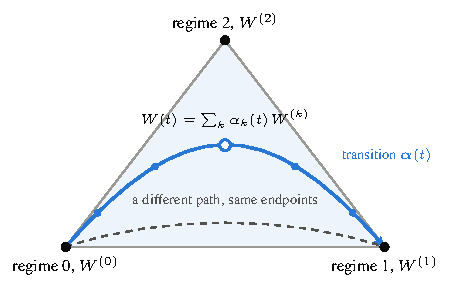
\includegraphics[width=0.82\columnwidth]{figs/concept.pdf}
\caption{A dynamic environment as a path in mechanism space. Each vertex is an atomic mechanism with its own transition matrix. A gradual transition is a path through the interior, described by time-varying mixing weights. A model with discrete regimes sees only the endpoints and cannot tell the two paths apart.}
\label{fig:simplex}
\end{figure}

% =====================================================================
\section{Background and Related Work}
\label{sec:related}

\para{Identifiability from change}
Nonlinear independent component analysis is not identifiable from i.i.d.\ data~\cite{hyvarinen1999nonlinear,locatello2019challenging}.
It becomes identifiable when an auxiliary variable modulates the distribution of the latents: nonstationarity~\cite{hyvarinen2016unsupervised}, temporal dependence~\cite{hyvarinen2017nonlinear}, or a general conditioning variable as in iVAE~\cite{hyvarinen2019nonlinear,khemakhem2020variational}.
The guarantee is always up to a permutation and a component-wise invertible map.

\para{Temporal CRL}
LEAP~\cite{yao2021learning} and TDRL~\cite{yao2022temporally} identify latent causal processes from time-delayed dependencies when the transition distribution varies enough across known domains.
NCTRL~\cite{song2023temporally} and CtrlNS~\cite{song2024causal} infer the domains instead of requiring labels.
Further work covers instantaneous effects~\cite{lippe2022icitris,li2024identification}, non-invertible mixing~\cite{chenlearning}, and sparsity of the latent mechanism~\cite{lachapelle2022disentanglement,zheng2022identifiability}.
All of these share the two limits discussed above.
The mechanism state is discrete, in line with causal discovery from nonstationary data~\cite{huang2020causal}.
The decoder is a dense network, so the model does not say which observed variables a latent controls.

\para{Modeling change over time}
Regime-switching state-space models~\cite{fox2011sticky} allow jumps between regimes but come without identifiability, and they do not parameterize intermediate states.
Mixture-of-experts models~\cite{jacobs1991adaptive,shazeer2017outrageously} combine specialized networks through a gate; we reuse this idea with one expert per atomic mechanism.

\para{Interpretable summaries of scientific time series}
VAMPnets~\cite{mardt2018vampnets}, TICA~\cite{perez2013tica}, and SPIB~\cite{wang2021state} produce low-dimensional summaries without identifiability and without an explicit map from latents to observed variables.
Sparse PCA~\cite{zou2006sparse} and ICA~\cite{hyvarinen2000independent} give readable loadings but are linear.
Sparse additive models~\cite{ravikumar2009sparse} provide the statistical tools we borrow for the decoder.

% =====================================================================
\section{Problem Setup}
\label{sec:problem}

\para{Generative model}
Observations $\vx_t\in\real^{D}$ are generated from latent factors $\vz_t\in\real^{n}$ by a smooth, injective mixing function $g$,
\begin{equation}
\vx_t = g(\vz_t) + \veps_t ,
\label{eq:mixing}
\end{equation}
with optional observation noise $\veps_t$.
The latents follow a lag-$L$ process whose transition law depends on a mechanism state $s_t$:
\begin{equation}
z_{t,j}\mid \vz_{t-L:t-1},\, s_t \;\sim\; p_j\!\left(\,\cdot \mid \vz_{t-L:t-1},\, s_t\right).
\label{eq:transition}
\end{equation}
A \emph{dynamic environment} is one in which $s_t$ varies with time.
In the simplest case $s_t$ is a regime label $c_t$ from a finite set.
More generally $s_t$ can move continuously between such regimes.

\para{Stage 1: identifiable latents}
Both parts of the project start from the same result.

\begin{theorem}[Latent identifiability]
\label{thm:latent}
Suppose the transition law~\eqref{eq:transition} varies sufficiently across regimes.
Then any representation $\hat\vz_t$ that explains the data and has conditionally independent components given the past satisfies $\hat z_i=h_i(z_{\pi(i)})$, where $\pi$ is a permutation and each $h_i$ is strictly monotonic.
\end{theorem}

This is the standard guarantee of temporal CRL~\cite{yao2022temporally}.
The argument writes $\hat\vz=\phi(\vz)$, applies the change-of-variables formula to the transition density, and uses conditional independence to force the mixed second derivatives of the log-density to vanish.
If the regimes differ in enough directions, the resulting linear system only admits a Jacobian of $\phi$ with one nonzero entry per row and column.
In practice Stage~1 is a sequential variational autoencoder whose prior over $\vz_t$ is a regime-conditioned transition model.

\para{Stage 2: two readouts}
Theorem~\ref{thm:latent} gives latents that are unique but tell us nothing about the environment.
The two aspects from the introduction become two estimation tasks on top of the frozen Stage~1 representation (Table~\ref{tab:compare}).
In tracking, we are given an unlabeled test sequence in which $s_t$ moves between regimes and must recover $s_t$.
In interpreting, we are given two regimes and must find the latent whose behavior differs most between them, together with the set of named observations it drives.

\begin{table}[t]
\centering
\footnotesize
\setlength{\tabcolsep}{4pt}
\begin{tabular}{@{}lll@{}}
\toprule
 & Tracking & Interpreting \\
\midrule
Goal & follow the transition & explain the change \\
Mechanism state & $\valpha(t)\in\Delta^{K-1}$ & regime $c_t\in\{0,1\}$ \\
Target & trajectory $\valpha(1{:}T)$ & supports $\cS_j\subseteq[D]$ \\
Structure used & convex combinations & additive main effects \\
Readout & least-squares projection & sparse additive decoder \\
Guarantee & Thms.~\ref{thm:pointwise}, \ref{thm:smooth} & Prop.~\ref{prop:nofp}, Thm.~\ref{thm:module} \\
\bottomrule
\end{tabular}
\caption{The two readouts built on the same identifiable latents.}
\label{tab:compare}
\end{table}

\begin{figure*}[t]
\centering
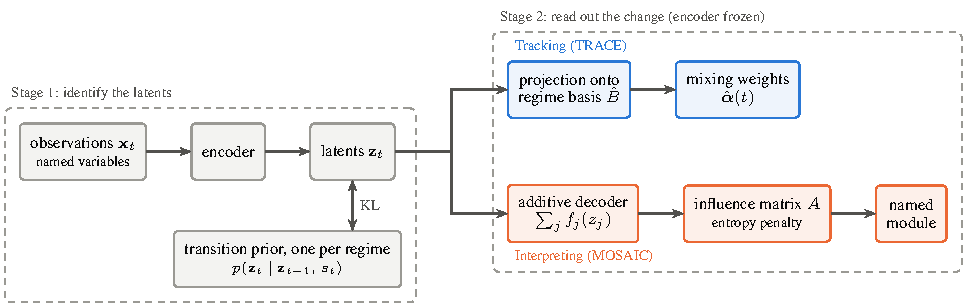
\includegraphics[width=\textwidth]{figs/pipeline.pdf}
\caption{Overview. Stage~1 learns identifiable latents with a regime-conditioned transition prior. Stage~2 freezes the encoder and adds one of two readouts: a projection that tracks the mixing weights of a transition, or an additive decoder whose influence matrix names the observed variables behind the latent that changes. Observed variables that behave differently in the two regimes are drawn in teal.}
\label{fig:pipeline}
\end{figure*}

% =====================================================================
\section{Tracking Mechanism Transitions}
\label{sec:track}

\subsection{Continuous mechanism states}

We describe a gradual transition with a small number of \emph{atomic mechanisms}.
The transition is $\vz_t=\sigma(W(t)\,\vz_{t-1})+\veps_t$ with a component-wise activation $\sigma$, and the transition matrix is a convex combination
\begin{equation}
W(t)=\sum_{k=0}^{K-1}\alpha_k(t)\,W^{(k)},\qquad \valpha(t)\in\Delta^{K-1},
\label{eq:convex}
\end{equation}
where $\Delta^{K-1}$ is the probability simplex (Fig.~\ref{fig:simplex}).
Each $W^{(k)}$ holds the causal edge strengths of one pure regime, and $\valpha(t)$ says how much of each regime is present at time $t$.
The same idea underlies mixing colors from primaries or documents from topics: a large space of mechanisms is described by a few anchors.

Training data come from the $K$ pure regimes, where $\valpha$ is a vertex.
At test time we see an unlabeled sequence that passes through the interior, and the goal is the whole trajectory $\valpha(1),\dots,\valpha(T)$.

\begin{assumption}[Distinguishable mechanisms]
\label{ass:distinct}
Write $\delta W^{(k)}=W^{(k)}-W^{(0)}$.
No $W^{(k)}$ is a convex combination of the others, and for each latent coordinate the corresponding rows of $\delta W^{(1)},\dots,\delta W^{(K-1)}$ are linearly independent.
This requires $K\le n+1$.
\end{assumption}

This assumption is what ``atomic'' means.
It also gives a concrete way to check the abstract variability condition of Theorem~\ref{thm:latent}: with Gaussian transition noise, the mixed derivative of the log transition density with respect to $z_{i,t}$ and $\vz_{t-1}$ is proportional to the $i$-th row of $W^{(k)}$, so linearly independent row differences translate directly into sufficient variability.

\subsection{Readout}

\para{Stage 1 as a mixture of experts}
A shared encoder maps observations to latents in every regime, which encodes the idea that the variables stay the same while their relations change (Fig.~\ref{fig:pipeline}).
Each regime $k$ has its own expert that models the transition as a normalizing flow, and a one-hot gate sends each training sample to its expert.
Training maximizes the usual evidence lower bound with the expert's transition model as the prior.

\para{Stage 2 as a projection}
Let $\hat\vmu^{(k)}$ be the conditional mean of the learned latent under regime $k$, computed on held-out data, and collect the shifts from a baseline regime in a matrix
$\hat B=[\hat\vmu^{(1)}-\hat\vmu^{(0)},\dots,\hat\vmu^{(K-1)}-\hat\vmu^{(0)}]$.
For a test observation with encoded latent $\hat\vz_t$,
\begin{equation}
\hat\valpha(t)=\mathrm{Proj}_{\Delta^{K-1}}\!\bigl(\hat B^{\dagger}(\hat\vz_t-\hat\vmu^{(0)})\bigr),
\label{eq:readout}
\end{equation}
followed by a moving average over a short window.
There is no gradient step at test time, so mixtures that never appeared in training are handled by construction.

\subsection{Recovery guarantees}

Let $\sigma_{\min}>0$ be the smallest singular value of $\hat B$ and $\epsilon=\max_k\|\delta W^{(k)}\|$.

\begin{theorem}[Pointwise recovery]
\label{thm:pointwise}
Under Theorem~\ref{thm:latent} and Assumption~\ref{ass:distinct}, the unprojected estimator in~\eqref{eq:readout} satisfies
\begin{equation}
\|\hat\valpha(t)-\valpha(t)\|\le\frac{1}{\sigma_{\min}}\bigl(\|\hat\veps_t\|+\delta_{\mathrm{approx}}\bigr),
\label{eq:pointwise}
\end{equation}
where $\hat\veps_t$ is the noise in the latent and $\delta_{\mathrm{approx}}=O(\epsilon^2)$.
\end{theorem}

\begin{proof}
By Theorem~\ref{thm:latent}, $\hat\vz=P\,h(\vz)$ with $P$ a permutation matrix and $h$ component-wise and monotonic.
Expanding $h$ to first order, the conditional mean of $\hat\vz_t$ under a mixture $\valpha$ is $\hat\vmu^{(0)}+\hat B\valpha+r(\valpha)$ with $\|r(\valpha)\|\le\delta_{\mathrm{approx}}$, and $\hat B=PD_hB$, where $B$ is the basis in the true latent space and $D_h$ is the Jacobian of $h$.
$D_h$ is diagonal because $h$ is component-wise; this is the only place where identifiability is needed.
Since $P$ and $D_h$ are invertible and $B$ has full column rank by Assumption~\ref{ass:distinct}, so does $\hat B$, hence $\hat B^{\dagger}\hat B=I$.
Applying $\hat B^{\dagger}$ to $\hat\vz_t-\hat\vmu^{(0)}=\hat B\valpha+r(\valpha)+\hat\veps_t$ gives
$\hat\valpha-\valpha=\hat B^{\dagger}r(\valpha)+\hat B^{\dagger}\hat\veps_t$, and $\|\hat B^{\dagger}\|=1/\sigma_{\min}$.
\end{proof}

The bound treats each time step on its own and does not improve with a longer sequence.
A transition is smooth, though, and smoothness helps.

\begin{theorem}[Smooth trajectory recovery]
\label{thm:smooth}
Assume the true trajectory has total variation at most $V$ and the noise is sub-Gaussian with parameter $\sigma$.
The estimator that minimizes the squared projection error plus $\lambda\sum_t\|\valpha_{t+1}-\valpha_t\|^2$, with $\lambda\asymp T^{1/3}$, has mean squared error
\begin{equation}
O\!\Bigl(\bigl(\tfrac{V}{T}\bigr)^{2/3}\frac{\sigma^{2/3}(K{-}1)^{1/3}}{\sigma_{\min}^{2/3}}+\frac{\delta_{\mathrm{approx}}^2}{\sigma_{\min}^2}\Bigr).
\end{equation}
\end{theorem}

The proof is a bias--variance argument.
The estimator is linear in the data, so its error splits into a bias from smoothing the true trajectory, a variance from the noise, and an approximation term.
A larger $\lambda$ increases the bias, which is controlled by $V$, and decreases the variance; balancing the two as for bounded-variation signals~\cite{tibshirani2014adaptive} gives the $T^{-2/3}$ rate.
The moving average in the readout is the practical version of this estimator.

Two remarks follow from the bound.
The recovered weights can be distorted in scale, but when $\epsilon^2/\sigma_{\min}$ is small the recovery map is monotone, so the shape and timing of a transition are preserved; a calibration at the two endpoints fixes the scale.
When the number of mechanisms that are active in a transition approaches $n+1$, the columns of $\hat B$ become nearly collinear and $\sigma_{\min}$ shrinks, so tracking degrades even if every atomic mechanism was learned correctly.

% =====================================================================
\section{Interpreting the Change}
\label{sec:interp}

Tracking tells us where the system is along a transition.
It does not tell us what is physically different between the two ends.
For that we fix two regimes, $c_t\in\{0,1\}$, which can be the endpoints of a transition or any contrast of interest such as folded versus unfolded.
The goal is to find the latent that differs most between the regimes and the observed variables that this latent drives.
The second part is what turns an anonymous coordinate into a named module.

\subsection{Supports of a latent}

``Drives'' needs a definition, because $g$ is not assumed additive and an observation may depend on several latents jointly.
We use the Hoeffding ANOVA decomposition~\cite{hoeffding1992class}.
Under a product reference measure $\mu=\prod_j\mu_j$ on the latents,
\begin{equation}
g(\vz)=g_0+\sum_{j=1}^{n}g_j(z_j)+r(\vz),
\label{eq:anova}
\end{equation}
with centered main effects $g_j$ and a remainder $r$ of higher-order interactions that is orthogonal to every function of a single coordinate.

\begin{definition}[Main-effect support]
\label{def:support}
$\cS_j=\{i\in[D]: g_j^{(i)}\text{ is non-constant}\}$, where $g_j^{(i)}$ is the $i$-th coordinate of $g_j$.
If the $\cS_j$ are disjoint they form a \emph{module partition} of the observed variables.
\end{definition}

\begin{proposition}[The additive fit finds the main effects]
\label{prop:nofp}
For any smooth $g$, let $\hat g(\vz)=\sum_j\hat f_j(z_j)+\hat\vb$ with centered $\hat f_j$ minimize $\E_\mu\|\vx-\hat g(\vz)\|^2$.
Then $\hat f_j=g_j$ for all $j$, and therefore $\hat\cS_j=\cS_j$.
\end{proposition}

\begin{proof}
Insert~\eqref{eq:mixing} and~\eqref{eq:anova} into the risk.
The noise is independent of $\vz$, and $r$ is orthogonal to all univariate functions, so no cross terms survive:
\begin{align}
\E_\mu\|\vx-\hat g(\vz)\|^2
&=\E\|\veps\|^2+\|g_0-\hat\vb\|^2+\E_\mu\|r(\vz)\|^2 \notag\\
&\quad+\sum_{j=1}^{n}\E_{\mu_j}\|g_j(z_j)-\hat f_j(z_j)\|^2 .
\end{align}
Each term of the sum is minimized separately at $\hat f_j=g_j$, and the interaction term cannot be reduced by any additive model.
\end{proof}

So an additive decoder fitted to a non-additive $g$ is not wrong for our purpose.
It converges to the main effects, and it never assigns a variable to a latent that has no main effect on it.
Variables that depend on a latent only through interactions are missed; that is the price of the additive target.

\begin{theorem}[Module identifiability]
\label{thm:module}
If $g$ is additive, two models that induce the same distribution over observations and regimes have the same supports up to a permutation of the latents.
With disjoint supports, the module partition is identifiable.
\end{theorem}

The proof has three short steps.
By Theorem~\ref{thm:latent}, the latents of the two models are related by a permutation and invertible maps $\phi_j$.
Both models have the same conditional mean of $\vx$, which gives two additive decompositions of the same function; since the centered decomposition is unique, the component functions agree up to composition with $\phi_j$ and a constant.
An invertible $\phi_j$ cannot turn a non-constant function into a constant one, so the supports match.
The same reasoning shows that the choice of the regime-associated latent is identifiable: we rank latents by the KL divergence between their distributions in the two regimes, and KL divergence is invariant under invertible maps.

For finite samples, classical results on sparse additive models~\cite{ravikumar2009sparse} apply to each observed variable separately.
Interactions act as additional noise, and the number of samples needed for support recovery scales with the ratio of noise plus interaction variance to the weakest main effect, with no dependence on the number of observed variables $D$.

\subsection{Readout}

After Stage~1, the encoder and the transition prior are frozen and the dense decoder is replaced by an additive head $\hat\vx=\sum_j f_j(z_j)+\vb$, where each $f_j$ is a small network (Fig.~\ref{fig:pipeline}).
With standardized latents we define the \emph{influence matrix}
\begin{equation}
A_{ij}=\bigl|f_j(+1)_i-f_j(-1)_i\bigr| ,
\end{equation}
which measures how much observation $i$ moves when latent $j$ moves.
To obtain modules we penalize the entropy of each normalized column,
\begin{equation}
\cL_{\text{sparse}}=\frac{1}{|\cJ_{\text{alive}}|}\sum_{j\in\cJ_{\text{alive}}}H\!\Bigl(A_{:,j}\big/\textstyle\sum_iA_{ij}\Bigr),
\end{equation}
where $\cJ_{\text{alive}}$ excludes latents that have collapsed.
The entropy is zero for a column with a single nonzero entry and $\log D$ for a uniform one, so the penalty pushes each latent toward a few observations without shrinking its overall effect.

At the end, latents are ranked by how much they shift between the two regimes; we use Cohen's $d$~\cite{cohen1988statistical} as a stable stand-in for the KL score.
The largest entries of the selected column name the latent.

% =====================================================================
\section{Experiments}
\label{sec:results}

Each part is compared with existing methods on one controlled benchmark and on real data.

\para{Metrics}
The mean correlation coefficient (MCC) is the average correlation between learned and true latents after Hungarian matching~\cite{kuhn1955hungarian}; it measures Stage~1.
Weight correlation is the Pearson correlation between true and recovered mixing trajectories.
Support precision is the fraction of a latent's three most influenced observations that lie in its true support, averaged over the three most regime-associated latents and counted only when those three entries hold at least half of the column mass.

\subsection{Tracking transitions}

\begin{figure*}[t]
\centering
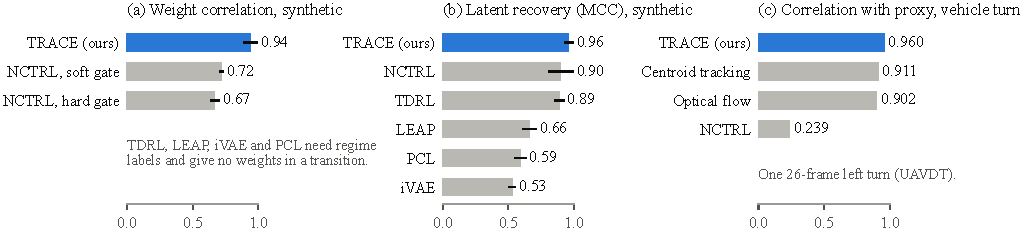
\includegraphics[width=\textwidth]{figs/track_results.pdf}
\caption{Tracking compared with existing methods. (a)~Correlation between recovered and true mixing weights on synthetic transitions. (b)~Latent recovery on the same benchmark. (c)~Correlation with a kinematic proxy on a real vehicle turn. Error bars show the spread across runs.}
\label{fig:track}
\end{figure*}

\para{Synthetic transitions}
The system has $n=8$ latents and $K=5$ atomic mechanisms, each differing from the baseline in one causal edge, so Assumption~\ref{ass:distinct} holds by construction.
Training uses the pure regimes only; test sequences move through three of them.
We compare with temporal CRL methods that assume discrete regimes: NCTRL~\cite{song2023temporally} with hard and soft gating, TDRL~\cite{yao2022temporally}, LEAP~\cite{yao2021learning}, PCL~\cite{hyvarinen2017nonlinear}, and iVAE~\cite{khemakhem2020variational}.
Figure~\ref{fig:track}(a) shows that our readout tracks the mixing weights with correlation $0.94$, against $0.72$ for NCTRL with soft gating.
The remaining methods require regime labels and cannot output anything during a transition.
Figure~\ref{fig:track}(b) shows that the shared encoder with one expert per regime also gives the best latents, with an MCC of $0.96$.
The raw weights have the right shape but a distorted scale; after calibration at the two endpoints, a path through three regimes, including its intermediate peak, matches the truth with correlation $0.99$.

\para{Real transitions}
For vehicle turns in the UAVDT aerial video dataset~\cite{Uavdt}, the two atomic mechanisms are horizontal and vertical motion, learned from vehicles driving straight.
There are no ground-truth weights, so we compare with a kinematic proxy, the share of the velocity in the vertical direction.
On a 26-frame left turn our readout reaches a correlation of $0.960$ with the proxy, and the recovered weight rises smoothly from $0$ to $1$ (Fig.~\ref{fig:track}(c)).
NCTRL reaches $0.239$ because it jumps back and forth between the two regimes.
Two simple heuristics based on centroid tracking and optical flow reach $0.911$ and $0.902$.
The same picture appears for walk-to-run transitions in motion-capture data with hip speed as the proxy: our readout reaches $0.856\pm0.043$ across trials, while NCTRL produces five spurious switches during a single transition.
The readout also works when the observations are images: on a CartPole system rendered as $128\times128$ frames, with five regimes that each strengthen one causal edge, it reaches an MCC of $0.970$ and a weight correlation of $0.95$ on a path through three regimes.

\subsection{Interpreting changes}

\begin{figure*}[t]
\centering
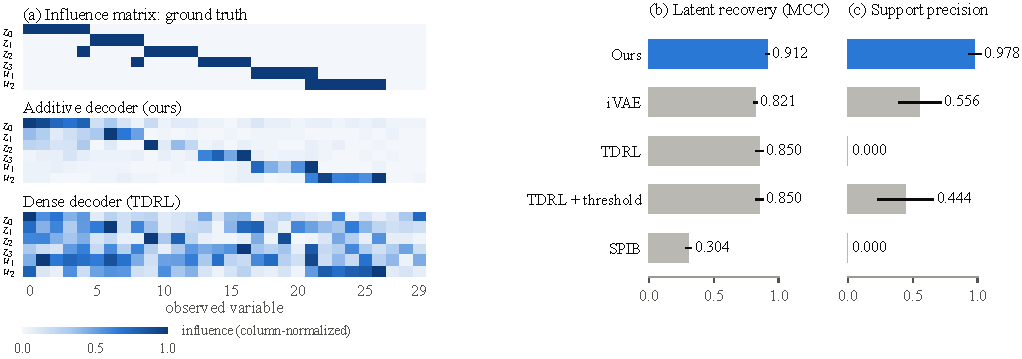
\includegraphics[width=\textwidth]{figs/interp_synth.pdf}
\caption{Interpretation on a benchmark with known supports. (a)~Influence of each true factor (rows) on each observed variable (columns): ground truth, our additive decoder, and a dense decoder. (b)~Latent recovery. (c)~Support precision. Error bars show one standard deviation over five seeds; the hatched bar is TDRL with its influence map thresholded after training.}
\label{fig:interp_synth}
\end{figure*}

\para{Benchmark with known supports}
A particle moves in a double-well energy landscape, and the well it occupies defines the regime.
Six latent factors generate thirty observations through monotonic nonlinear mixing, and some observations are deliberately shared between factors.
The baselines are iVAE, TDRL, TDRL with its influence map thresholded after training, and SPIB~\cite{wang2021state}.
Figure~\ref{fig:interp_synth}(a) shows that our decoder recovers the block structure of the true influence matrix, while the dense decoder of TDRL spreads the influence of every latent over all observations.
The numbers agree.
The CRL methods all recover reasonable latents (Fig.~\ref{fig:interp_synth}(b)), but only our decoder reaches a high support precision, $0.978$ (Fig.~\ref{fig:interp_synth}(c)).
TDRL scores zero, and thresholding its influence map afterwards only reaches $0.444$, so sparsity has to be learned together with the additive structure.

\begin{figure*}[t]
\centering
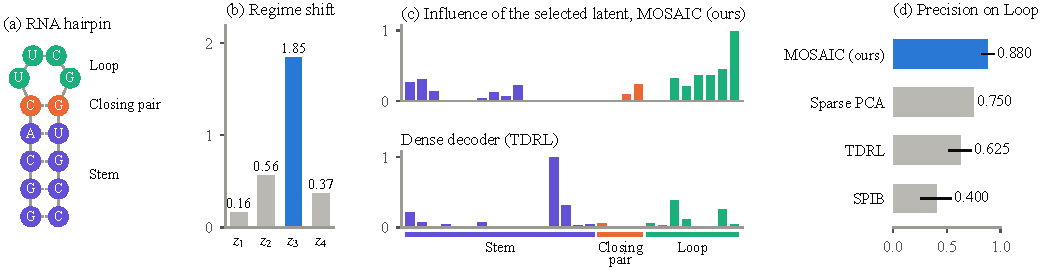
\includegraphics[width=\textwidth]{figs/interp_rna.pdf}
\caption{An RNA hairpin. (a)~The molecule and its three structural regions. (b)~Regime shift (Cohen's $d$) of each learned latent; $z_3$ is selected. (c)~Influence of the selected latent on each of the 28 features, for our decoder and for a dense decoder. (d)~Precision of the eight most influenced features against the Loop.}
\label{fig:interp_rna}
\end{figure*}

\para{RNA hairpin}
We use molecular dynamics of a 14-nucleotide RNA hairpin simulated at three temperatures (Fig.~\ref{fig:interp_rna}(a)).
Each frame is described by $D=28$ per-residue distance features, which belong to three structural regions (Stem, Closing Pair, Loop); the region labels are never shown to the model.
The two regimes are defined by whether the closing base pair is intact.
One latent, $z_3$, stands out in its regime shift (Fig.~\ref{fig:interp_rna}(b)), and its influence concentrates on Loop features (Fig.~\ref{fig:interp_rna}(c)).
This agrees with what is known about this molecule, where fluctuations of the loop couple to the opening of the closing pair~\cite{chen2013rna}.
The dense decoder also produces a sparse-looking profile, but its largest entry is in the Stem.
Measured as the precision of the eight most influenced features against the Loop, our decoder reaches $0.880$, Sparse PCA $0.750$, TDRL $0.625$, and SPIB $0.400$ (Fig.~\ref{fig:interp_rna}(d)).

\begin{figure*}[t]
\centering
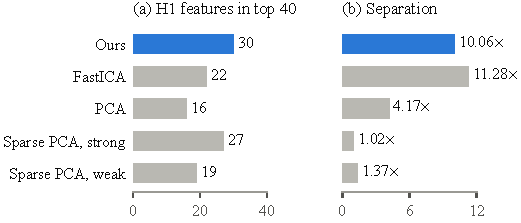
\includegraphics[width=\textwidth]{figs/interp_protein.pdf}
\caption{A three-helix protein and four further domains. (a)~Number of the 40 most influenced features that lie in helix H1, which holds 40 of the 132 features; the dashed line is the chance level. (b)~Ratio between the largest and second-largest regime shift among components. SPCA is Sparse PCA with a strong or a weak penalty. (c)~Ratio between the mean influence on the expected group of variables and on the runner-up group, shown as the range over three runs per domain. The expected group ranked first in all runs.}
\label{fig:interp_protein}
\end{figure*}

\para{Protein}
The second molecular system is the three-helix protein HP35, from a long folding simulation~\cite{piana2012protein}.
Each frame is described by 132 backbone dihedral angles, and the regimes are defined by whether the first helix, H1, is folded.
The model sees the angles and the regime label, with no information about which angles belong to H1.
Figure~\ref{fig:interp_protein}(a,\,b) shows that simple baselines get either a clearly separated component or a localized one.
FastICA separates well but its features are spread over the protein, and Sparse PCA with a strong penalty concentrates on H1 but cannot tell H1 from H2.
Our decoder gives a clearly separated latent with 30 of its top 40 features in H1.

\para{Other domains}
With the same pipeline and hyperparameters we also tried solar wind~\cite{king2005omni}, sea-surface temperature with ENSO phases~\cite{huang2017extended}, the Tennessee Eastman chemical process~\cite{downs1993plant}, and a synthetic tokamak benchmark.
No latent ground truth exists there, so we only checked whether the group of variables with the largest mean influence is the one that domain knowledge expects.
It was in all 12 runs.
Figure~\ref{fig:interp_protein}(c) shows how clearly the expected group stands out.
Its mean influence is up to twice that of the runner-up group for the tokamak and climate data, and close to it for the chemical process, where four different faults are labeled as one regime and share a single downstream signature.

\subsection{A compact implementation}
\label{sec:own}

\begin{figure*}[t]
\centering
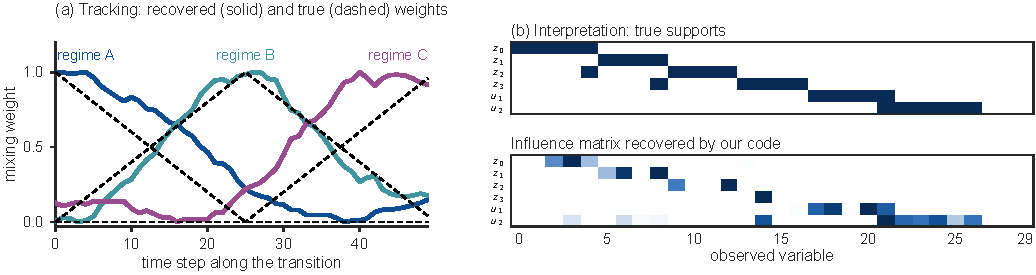
\includegraphics[width=\textwidth]{figs/own_runs.pdf}
\caption{Runs of our compact implementation on a laptop CPU. (a)~Mixing weights along a path through three of five regimes, recovered after endpoint calibration (solid) and true (dashed). (b)~True supports of the double-well benchmark and the influence matrix recovered by the additive decoder. Each row shows the learned latent matched to that factor, normalized by its maximum.}
\label{fig:own}
\end{figure*}

The experiments above were run at full scale on GPUs.
To check that the two readouts do not depend on that scale, we wrote a compact implementation of the shared first stage and of both readouts in a few hundred lines of PyTorch.
It simulates its own data and runs on a laptop CPU in about ten minutes per experiment.
For tracking, the model is trained on $20{,}000$ windows from each of five regimes and tested on a path through three of them.
It reaches an MCC of $0.970$ and a weight correlation of $0.967$ after smoothing, against $0.874$ before, and Fig.~\ref{fig:own}(a) shows the recovered path.
For interpretation, the double-well system is simulated with 32 short chains, about a quarter of the data used above.
The model reaches an MCC of $0.943$ and a support precision of $0.889$.
The three latents with the largest regime shift are matched to the three factors that drive the regime, and the recovered influence matrix follows the block structure of the true supports (Fig.~\ref{fig:own}(b)).
The recovered supports are sparser than the true ones: every latent finds a part of its block rather than all of it.

% =====================================================================
\section{Discussion}
\label{sec:discussion}

\para{A shared design}
Both parts split the problem into a hard part that existing theory already covers and a new part that is kept simple.
The hard part is identifying the latents from regime-dependent dynamics.
The new part is a readout from the frozen representation: the shift of the encoder's conditional mean for tracking, the decoder for interpretation.
The two proofs also have the same shape.
Identifiability says the learned latent equals the true one up to a permutation and a component-wise map, and the proof shows that the readout does not care about this ambiguity.
For tracking, a component-wise map contributes a diagonal Jacobian, which does not change the rank of the basis.
For interpretation, it cannot turn a non-constant main effect into a constant one.

\para{Relation between the two parts}
The two readouts describe complementary sides of the same change.
Tracking places the system on a path between regimes but says nothing about which observed quantities are involved.
Interpretation names the quantities involved but handles one contrast between two regimes at a time.
Used together, one would first locate a transition in time and then determine what distinguishes its two ends.

\para{Limitations}
Tracking needs labeled data from the pure regimes and the number of atomic mechanisms, and it is restricted to convex combinations.
Interpretation misses variables that depend on a latent only through interactions, and a weak signal from the same source as a strong one can be split off into a separate latent.
The sparsity penalty we use has no finite-sample guarantee yet; the available one covers a group-lasso estimator.

\para{Lessons learned}
(1)~Identifiability is a means.
A latent that is unique but unnamed, or a regime label that is discrete when the process is not, is not yet useful to a scientist.
(2)~A simple readout is worth more than a flexible one, because it can be analyzed.
Both central proofs are a few lines once the right decomposition is in place.
(3)~A bound is most useful when it names what limits performance; the tracking bound says directly that mechanisms must be distinct enough relative to the noise.
(4)~Sparsity is not interpretability.
On the RNA data a dense decoder also produced a concentrated profile, in the wrong place.
(5)~Without ground truth, claims should be made at the resolution of the evidence.

% =====================================================================
\section{Conclusions and Future Work}
\label{sec:conclusion}

We studied causal representation learning in environments whose mechanisms change over time, and examined what can be recovered about the change itself once the latents are identified.
For the transition, we modeled it as a convex combination of atomic mechanisms and showed that the mixing trajectory is recovered by a least-squares readout with an explicit error bound and a better rate for smooth trajectories.
For the meaning of the change, we showed that the supports of the latents over named observations are identifiable through an additive decoder, which turns the latent that moves with the regime into a physical module.
Controlled experiments agree with the theory, and results on vehicle motion and molecular dynamics are consistent with it.

\para{Future work}
The natural next step is to join the two readouts: replace the binary regime in the interpretation part by the recovered trajectory $\valpha(t)$, so that the observed variables that change along a gradual transition can be identified.
The projection and the additive decoder act on different parts of the model, so this is possible in principle; what remains open is whether supports stay identifiable when the conditioning variable is itself estimated.
Other directions are a finite-sample guarantee for the entropy penalty, learning the atomic mechanisms from unlabeled transitions, a second-order decoder that captures pairwise interactions, and real datasets with partial ground truth for supports or mixing weights.

% =====================================================================
\section*{Team Contributions}
All three members worked out the problem formulation and went through the proofs together.
Shicheng Fan implemented the shared first stage and the interpretation readout (Sec.~\ref{sec:interp}), ran its experiments, and integrated the two parts in the code and in this report.
Jie Yang worked on the tracking part (Sec.~\ref{sec:track}): the transition paths of the synthetic benchmark, the discrete-switching baseline, and, together with Shicheng Fan, the tracking experiments.
Honghui Bao wrote the intermediate report, the literature survey (Sec.~\ref{sec:related}), and the problem setup (Sec.~\ref{sec:problem}), and extended the compact implementation (Sec.~\ref{sec:own}) with the dense-decoder baseline for the interpretation readout, the unit tests, and the plots of the influence matrices.

The proposal, both reports, and the code are maintained at \url{https://github.com/shichengf/CS412}.

\nocite{fan2026mosaic,fan2026trace}
{
    \footnotesize
    \bibliographystyle{ieeenat_fullname}
    \bibliography{refs}
}

\end{document}
